\documentclass[a4paper,12pt]{article}

\input{preamble}

\begin{document}

\begin{titlepage}
    \begin{center}
        % NTU Logo
        \includegraphics[width=0.7\textwidth]{figs/NTUlogo.png} 
        \\[2cm]
        
        {\huge \textbf{Quantum State Tomography of an Entangled Two-qubit System}} 
        \\[2cm]
        
        {\large \textbf{Oscar Stommendal}} 
        \\[0.2cm]
        
        {\large \href{mailto:N2402294F@e.ntu.edu.sg}{\textsc{N2402294F@e.ntu.edu.sg}}}
        \\[2cm]
        
        {\textbf{SCHOOL OF PHYSICAL AND MATHEMATICAL SCIENCES}} 
        \\[2cm]
        
        {\Large PH3406 Open Quantum Systems} 
        \\[0.5cm]
        
        {\Large \textbf{Project Report}} 
        \\[2cm]

        % \DTMlangsetup{showdayofmonth=false}
        \vfill
        {\Large \today}
    \end{center}
\end{titlepage}

\section{Introduction}
The last decade, the field of quantum information and computing has seen rapid development. Quantum computers have showed the potential to outperform classical computers in certain tasks, and many believe that we are on the edge of a quantum revolution \cite{outperform} \cite{revolution}. In December 2024, several publicly traded companies within the quantum computing area reached new records in share prices \cite{rocket}. So, the interest in quantum computing is growing, also outside of academia, and the field is attracting more and more attention. 

However, the technology is still in its first phase, and faces many challenges \cite{challenge}. These include the need for error correction due to noise, upscaling of the number qubits and hardware development. In this report, we will focus on \textit{quantum state tomography} (QST). This is a method used to characterize the state of a quantum system, which has several important applications within quantum computing, for example in error correction.

\section{Theory}
This section provides the necessary background to understand the rest of the report. We will start by introducing the basic concepts of quantum computing, followed by a more detailed explanation of QST.
\subsection{Introduction to Open Quantum Systems}
When studying closed systems within quantum mechanics, we describe the system by a state vector $\ket{\psi}$, which evolves in time according to the Schrödinger equation,
\begin{equation}
    i\hbar \frac{d}{dt} \ket{\psi} = \hat{H} \ket{\psi}.
\end{equation}
Here, $\hat{H}$ is the Hamiltonian, which describes the energy of the system. However in reality, no system is completely isolated, and we must consider the interaction with the environment. This leads to the concept of open quantum systems, where the system state is described by a density matrix $\hat{\rho}$ \cite{nielsen_chuang}. This matrix is essentially a generalization of the state vector, and contains the same information, with the difference that it can also describe mixed states. Mixed states are states that are not pure (like the ones in closed systems), but rather a statistical mixture of pure states. The density matrix is defined as
\begin{equation}
    \hat{\rho} = \sum_i p_i \ket{\psi_i} \bra{\psi_i},
\end{equation}
where $p_i$ is the probability of the system being in the state $\ket{\psi_i}$. When performing QST, we are essentially trying to reconstruct this density matrix from measurements of the system. An appropriate measure to test the result of the tomography is the so called \textit{fidelity}, which is a measure of how close the reconstructed state is to the ideal state $\hat{\rho}$. The fidelity is defined as
\begin{equation} \label{fid}
    \mathcal{F}(\hat{\rho}, \hat{\rho}_{\text{exp}}) = \text{Tr}\left(\sqrt{\sqrt{\hat{\rho}}\hat{\rho}_{\text{exp}}\sqrt{\hat{\rho}}}\right ),
\end{equation}
where $\hat{\rho}_{\text{exp}}$ is the reconstructed state and Tr() the trace \cite{nielsen_chuang}. If $\mathcal{F}$ is equal to 1, the reconstructed state is identical to the ideal state, and if it is 0, the states are orthogonal.
% \subsection{Introduction to Quantum Computing}
% As the introduction suggested, the quantum computing field is growing rapidly. One part of the reason for this is the potential of quantum computers to outperform classical computers in certain tasks. Contrary to classical computers, which processes data through bits that can be either 0 or 1, quantum computers use quantum bits, or \textit{qubits}. Mathematically, we express these as a vector in a two-dimensional Hilbert space, $\mathcal{H}$, according to
% \begin{equation}
%     \ket{\psi} = \alpha \ket{0} + \beta \ket{1},
% \end{equation}
% where $\alpha$ and $\beta$ are complex numbers, and $\ket{0}$ and $\ket{1}$ are the basis states of the qubit. The state $\ket{\psi}$ is normalized, meaning that $|\alpha|^2 + |\beta|^2 = 1$.
\subsection{Quantum State Tomography}
In quantum mechanics, the state of the considered system is usually of highest interest, as this contains all the system information. However, due to the nature of quantum mechanics, once we measure the outcome of a system, the state collapses to one of the possible outcomes \cite{nielsen_chuang}. So, the root of the problem considered in this project is that no measurement can differentiate between non-orthogonal states like $\ket{0}$ and $\frac{1}{\sqrt{2}}(\ket{0} + \ket{1})$. This means that we cannot measure the state directly, but rather have to reconstruct it from repeated measurements of the system. This is where QST comes into play.

The basic idea of QST is to prepare the system in the same way many times and measure the outcome. The density matrix $\hat{\rho}$ is then reconstructed from the measurement data. In principle, the measurements are done using the Pauli operators, which together with the identity operator form a basis for the space of operators \cite{nielsen_chuang}. By measuring the outcome of these different basis operators many times, the density matrix can be reconstructed. For example, in the case of one qubit, $\hat{\rho}$ can be written as
\begin{equation}
    \hat{\rho} = \frac{1}{2}\left(\mathbb{I} + \sum_{i=1}^3 \langle \sigma_i\rangle \sigma_i\right),
\end{equation}
where $\mathbb{I}$ is the identity matrix, $\sigma_i$ are the Pauli operators and $\langle \sigma_i\rangle$ are the expectation values of the Pauli operators. This can then be generalized to more qubits.
\section{Methodology}
The foundation of the method in this project is taken from \href{https://qiskit-community.github.io/qiskit-experiments/manuals/verification/state_tomography.html}{Qiskit's} experiment manual on QST. Some adjustments have been made to the code, in order to fit the specific goals here. The code is written in \texttt{Python} and uses the \texttt{Qiskit} library for creating and transpiling circuits, the \texttt{Qiskit Aer} library for simulating the problems with noise and the \texttt{Qiskit Experiments} library for performing the state tomography \cite{qiskit} \cite{qiskit_aer} \cite{qiskit_exps}. For reference, the complete source code is available on \href{https://github.com/stommen/ntu_exchange/tree/main/ntu_courses/PH3406}{GitHub}.

\subsection{Quantum Circuit}
The quantum state used in this project is an entangled two-qubit system, initialized using the circuit in Figure \ref{fig:entangled_circuit} below.

\begin{figure}[h!]
    \centering
    \begin{quantikz}
        \lstick{$\ket{0}$} & \gate{H} & \gate{S} & \ctrl{1} & \qw \\
        \lstick{$\ket{0}$} & \qw      & \qw      & \targ{}  & \qw
    \end{quantikz}
    \caption{The quantum circuit used to initialize an entangled two-qubit system. Note that the input state is $\ket{00}$. This figure was created using the \texttt{quantikz} package \cite{quantikz}.}
    \label{fig:entangled_circuit}
\end{figure}

The circuit consists of a Hadamard gate, an S gate and a CNOT gate. The Hadamard gate puts the first qubit in a superposition state between $\ket{0}$ and $\ket{1}$ and the S gate gives an extra phase of $\sfrac{\pi}{2}$ to the state $\ket{1}$. Lastly, the CNOT with target on the second qubit will change this from 0 to 1 if the first qubit is in state $\ket{1}$. Thus, with input state $\ket{00}$ on an ideal quantum computer, this circuit will produce the state
\vspace{-0.3cm}
\begin{equation}\label{state}
    \ket{\psi} = \frac{1}{\sqrt{2}}(\ket{00} + i\ket{11}) \equiv \frac{1}{2}\begin{bmatrix}
        1 & 0 & 0 & -i \\
        0 & 0 & 0 & 0 \\
        0 & 0 & 0 & 0 \\
        i & 0 & 0 & 1
    \end{bmatrix} = \hat{\rho}.
\end{equation}
In \texttt{Qiskit}, this is easily implemented according to the code snippet below.

\begin{tcolorbox}[title = {\footnotesize\textbf{Code Snippet, Quantum Circuit}}, colback=black!15!white, colframe=black]
    \begin{adjustwidth}{0.25cm}{0cm}
    
    {\footnotesize 
    \begin{minted}[linenos,breaklines]{python}
    # State preparation circuit 
    qc = qiskit.QuantumCircuit(2, 2) # Create a quantum circuit with 2 qubits (the other argument is for the classical register, not used in the state tomography)
    qc.h(0) # Apply a Hadamard gate on the first qubit
    qc.s(0) # Apply an S gate on the first qubit
    qc.cx(0, 1) # Apply a CNOT gate between the first and second qubit
    \end{minted}
    }
    \end{adjustwidth}
\end{tcolorbox}

\subsection{Noise Modelling}
In order to get more realistic results, some experiments will be run with noise, as this is a common problem in quantum computing. Noise can come from several sources, such as the environment or the hardware, and can affect the qubits in different ways \cite{nielsen_chuang}. In this project, we focus on two noise models: \textit{depolarizing noise} and \textit{measurement noise}. The depolarizing noise basically replaces the original state with the maximally mixed state, $\hat{\rho}_M = \alpha\mathbb{I}$ to some degree, as we will see later \cite{nielsen_chuang}. The measurement noise, on the other hand, is a type of noise that occurs when the measurement of the qubit is not perfect, and the result is not always correct. These two models are especially interesting in QST as they affect the resulting state, which is what we are trying to reconstruct. Below follows a brief explanation of how the noise models were implemented in \texttt{Qiskit} together with some theoretical background on the models. 

\subsubsection{Depolarizing Noise}
The depolarizing noise is added by applying a depolarizing error (or channel) to each gate in the circuit. The code snippet below shows how to implement this in \texttt{Qiskit}.

\begin{tcolorbox}[title = {\footnotesize\textbf{Code Snippet, Depolarizing Noise Model}}, colback=black!15!white, colframe=black]
    \begin{adjustwidth}{0.25cm}{0cm}
    
    {\footnotesize 
    \begin{minted}[linenos,breaklines]{python}
    p = 0.1 # Error probability
    error_1 = depolarizing_error(p, 1) # 1-qubit gate error
    error_2 = depolarizing_error(p, 2) # 2-qubit gate error

    # Add errors to noise model
    noise_model = NoiseModel() # Create a noise model
    noise_model.add_all_qubit_quantum_error(error_1, ['h', 's']) # Add 1-qubit gate errors to the noise model
    noise_model.add_all_qubit_quantum_error(error_2, ['cx']) # Add 2-qubit gate errors to the noise model

    noise_backend = AerSimulator(noise_model=noise_model) # Noise simulator
    trans_qc = transpile(qc, noise_backend) # Transpile the circuit to the noise model (in order to apply the noise)
    \end{minted}
    }
    \end{adjustwidth}
\end{tcolorbox}

Here, the error rate is given by a parameter $p$, which is the probability of an error occurring \cite{nielsen_chuang}. Mathematically, the state after the depolarizing error is given by
\begin{equation} \label{depolarizing}
    \mathcal{D}(\hat{\rho}) = \frac{p\,\mathbb{I}_d}{d} + (1-p)\hat{\rho},
\end{equation}
where $\mathbb{I}_d$ is the identity matrix in dimension $d$. Studying the code example above, for the Hadamard and S gate, $d=2$ and for the CNOT gate, $d=4$. This means that the state is mapped to a linear combination of the original state and the maximally mixed state $\hat{\rho}_{mixed} = \sfrac{\mathbb{I}}{d}$. During the experiments, the value $p = 0.1$ was used.

\subsubsection{Measurement Noise}
The measurement noise is added by creating a readout error object, which is added to the noise model. This error object is a matrix that describes the probability of the measurement being correct or incorrect. For one qubit, this is the $2 \times 2$ matrix
\begin{equation}
    \epsilon = \begin{bmatrix}
        \mathcal{P}(0|0) & \mathcal{P}(0|1) \\
        \mathcal{P}(1|0) & \mathcal{P}(1|1)
    \end{bmatrix}.
\end{equation}
So, the diagonal elements are the probabilities of the correct measurement, and the off-diagonal elements are the probabilities of incorrect measurements. In the experiments, a probability of $\mathcal{P}(0|0) = \mathcal{P}(1|1) = 0.9$ for the correct measurement and $\mathcal{P}(0|1) = \mathcal{P}(1|0) = 0.1$ for the incorrect measurement was used (for a more fair comparison, this is the same error probability as for the depolarizing noise). The code snippet below shows how to implement this in \texttt{Qiskit}. One could have added this error when measuring both qubits simultaneously, but for simplicity, we consider the error on each qubit separately. 

\begin{tcolorbox}[title = {\footnotesize\textbf{Code Snippet, Measurement Noise Model}}, colback=black!15!white, colframe=black]
    \begin{adjustwidth}{0.25cm}{0cm}
    
    {\footnotesize 
    \begin{minted}[linenos,breaklines]{python}
    probs = np.zeros((Nq, Nq)) # Create an error probability matrix, with Nq being the number of qubits
    for i in range(0, Nq):
        for j in range(0, Nq):
            if i == j:
                probs[i, j] = 0.9 # Probability of correct measurement
            else:
                probs[i, j] = 0.1 # Probability of incorrect measurement

    readout_error = ReadoutError(probs) # Create a readout error object
    
    noise_model = NoiseModel() # Create a noise model
    noise_model.add_all_qubit_readout_error(readout_error) # Add the error to both qubits
    
    noise_backend = AerSimulator(noise_model=noise_model) # Noise simulator
    trans_qc = transpile(qc_ghz, noise_backend) # Apply the noise
    \end{minted}
    }
    \end{adjustwidth}
\end{tcolorbox}

\subsection{Quantum State Tomography}
When performing QST, we use the \lstinline|StateTomography| class in the \texttt{Qiskit Experiments} library \cite{qiskit_exps}. This takes the quantum circuit as input, and returns a result object that for example contains the reconstructed density matrix and the fidelity between the ideal and the reconstructed state. The code snippet below shows the implementation.

\begin{tcolorbox}[title = {\footnotesize\textbf{Code Snippet, Quantum State Tomography}}, colback=black!15!white, colframe=black]
    \begin{adjustwidth}{0.25cm}{0cm}
    
    {\footnotesize 
    \begin{minted}[linenos,breaklines]{python}
    backend, qc = get_QST_qc(Nq, noise=noise, noise_choice=noise_choice) # Get the circuit and backend

    qst = StateTomography(qc) # Create a state tomography object
    qst_data = qst.run(backend=backend, shots=counts).block_for_results() # Run the state tomography
    \end{minted}
    }
    \end{adjustwidth}
\end{tcolorbox}

In the code above, \lstinline|get_QST_qc()| is a function that returns the quantum circuit and the backend, depending on the noise model chosen. If the experiment is performed without noise, specified by setting the variable \mintinline{python}|noise=False|, the default \lstinline|AerSimulator()| backend is used. The \lstinline|noise_choice| parameter is used to choose between the two noise models, and the \lstinline|counts| parameter is the number of measurements taken. During the experiments, a fixed value of \lstinline|counts |$= 10\,000$ were used. For the input system $\ket{\psi}$ in Equation \ref{state}, the tomography was performed 4 times -- one time without noise, one with depolarizing noise, one with measurement noise and one with both noise models.

\subsubsection{Alternative Tomography Fitters and Parallel Experiments}
Except for the experiments described above, some additional experiments were performed. Firstly, one was done to compare the performance of different tomography fitters, which are the algorithms used to reconstruct the density matrix $\hat{\rho}$ from the measurement data. The fitters used in this project are \lstinline|linear_inversion| and \lstinline|cvxpy_gaussian_lstsq|. The first one is a least squares fitter, while the second one is a more advanced fitter (of the same type) that uses constrains on $\hat{\rho}$ to ensure that it is positive semidefinite (i.e. that it has non-negative eigenvalues) \cite{qiskit_exps}. The first fitter also ensures this, however by executing some extra calculations. Using \texttt{Qiskit}, the fitter can be set by adding the line

{\footnotesize 
\begin{minted}[breaklines]{python}
    qst.analysis.set_options(fitter='cvxpy_gaussian_lstsq')
\end{minted}
}

between line 3 and 4 in the code above. The fitters were then tested on $\ket{\psi}$ in Equation \ref{state} subject to both depolarizing and measurement noise implemented as before.

Secondly, a so called parallel experiment was performed. As the name suggests, this is an experiment which runs several sub-experiments in parallel. As QST gets more time-consuming with increasing number of qubits, this could be a way to save time \cite{nielsen_chuang}. In this case, the experiment was done on a circuit with 5 qubits, shown in Figure \ref{fig:5qubit_circuit} below.

\begin{figure}[H]
    \centering
    \begin{quantikz}
        \lstick{$\ket{0}$} & \gate{H} & \qw & \qw & \qw & \qw \\
        \lstick{$\ket{0}$} & \qw & \ctrl{2} & \qw & \qw & \qw \\
        \lstick{$\ket{0}$} & \qw & \qw & \gate{S} & \qw & \qw \\
        \lstick{$\ket{0}$} & \qw & \targ{} & \qw & \qw & \qw \\
        \lstick{$\ket{0}$} & \qw & \qw & \qw & \gate{X} & \qw
    \end{quantikz}
    \caption{The 5-qubit quantum circuit used in the parallel experiments. Note that the input state is $\ket{00000}$. This figure was created using the \texttt{quantikz} package \cite{quantikz}.}
    \label{fig:5qubit_circuit}
\end{figure}

The parallel experiment was done with depolarizing noise, implemented as before. The code snippet below shows how to implement the parallel experiment (with the \mintinline{python}|backend| variable being the depolarizing noise backend). Similar to before, a number of \mintinline{python}|counts |$=10\,000$ shots were used together with the \mintinline{python}|linear_inversion| fitter. The reconstructed density matrices were then plotted and compared to the ideal state via the fidelity.

\begin{tcolorbox}[title = {\footnotesize\textbf{Code Snippet, Parallel Experiments}}, colback=black!15!white, colframe=black]
    \begin{adjustwidth}{0.25cm}{0cm}
    
    {\footnotesize 
    \begin{minted}[linenos,breaklines]{python}
    gates = [qiskit.circuit.library.HGate(), qiskit.circuit.library.SGate(), qiskit.circuit.library.CXGate(), qiskit.circuit.library.XGate()] # Gates in the circuit

    subexps = [StateTomography(gates[0], physical_qubits=(0, )), StateTomography(gates[1], physical_qubits=(2, )), StateTomography(gates[2], physical_qubits=(1, 3)), StateTomography(gates[3], physical_qubits=(4, ))] # QST sub-experiments

    # Create and run a parallel experiment
    parexp = ParallelExperiment(subexps, flatten_results=False)
    pardata = parexp.run(backend, shots=10000).block_for_results()
    \end{minted}
    }
    \end{adjustwidth}
\end{tcolorbox}
\vspace{-0.2cm}
\section{Results}
Below follows the results from the experiments with and without noise for the QST with different fitters, along with the parallel experiments. Note that, unlike \texttt{Qiskit's} experimental manual on this topic, the axis labels also include the braket notation.

\subsection{Without Noise}
Figure \ref{fig:ideal} shows the reconstructed density matrix $\hat{\rho}$ of the entangled two-qubit system after performing the QST without noise. The fidelity between the ideal and the reconstructed state was $\mathcal{F} = 0.9966$. 
\begin{figure}[H]
    \centering
    \includegraphics[width=0.9\textwidth, trim={6cm 5cm 3cm 3cm},clip]{figs/density_matrix_ideal.pdf}
    \caption{The reconstructed density matrix $\hat{\rho}$ of the entangled two-qubit system after performing the quantum state tomography without noise.}
    \label{fig:ideal}
\end{figure}
\vspace{-0.7cm}
\subsection{With Noise}
Table \ref{tab:noise} shows the fidelity and fitting time after performing the QST with depolarizing noise, measurement noise and both noise models for different tomography fitters. The corresponding reconstructed density matrices $\hat{\rho}$ with the different noise models are shown in Figures \ref{fig:depol}, \ref{fig:meas} and \ref{fig:both}, respectively. Note that the fidelity is significantly lower when noise is added to the system and that no figures are shown for the \mintinline{python}|cvxpy_gaussian_lstsq| fitter, as we essentially only need the fidelity to compare the different fitters.
\begin{table}[H]
    \centering
    \caption{The fidelity $\mathcal{F}(\hat{\rho}, \hat{\rho}_{\text{exp}})$ and fitting time after performing the quantum state tomography with depolarizing noise, measurement noise and both noise models for different tomography fitters.}
    \begin{tabular}{|l|c|c|c|}
        \toprule
        \textbf{Noise Model(s)} & \textbf{Tomography Fitter} & \textbf{Fidelity $\mathcal{F}(\hat{\rho}, \hat{\rho}_{\text{exp}})$} & \textbf{Fitting Time} \\
        \midrule
        Depolarizing & \mintinline{python}|linear_inversion| & 0.7689 & 0.0062 \\
        Measurement & \mintinline{python}|linear_inversion| & 0.7308 & 0.0046 \\
        Both & \mintinline{python}|linear_inversion| & 0.5777 & 0.0056 \\ \midrule
        Depolarizing & \mintinline{python}|cvxpy_gaussian_lstsq| & 0.7726 & 0.0355 \\
        Measurement & \mintinline{python}|cvxpy_gaussian_lstsq| & 0.7330 & 0.0239 \\ \bottomrule
    \end{tabular}
    \label{tab:noise}
\end{table}
\vspace{-1cm}
\begin{figure}[H]
    \centering
    \includegraphics[width=0.9\textwidth, trim={6cm 5cm 3cm 2cm},clip]{figs/density_matrix_depol.pdf}
    \caption{The reconstructed density matrix $\hat{\rho}$ of the entangled two-qubit system after performing the quantum state tomography with depolarizing noise. In this case, the \texttt{linear\_inversion} fitter was used.}
    \label{fig:depol}
\end{figure}
\vspace{-1cm}
\begin{figure}[H]
    \centering
    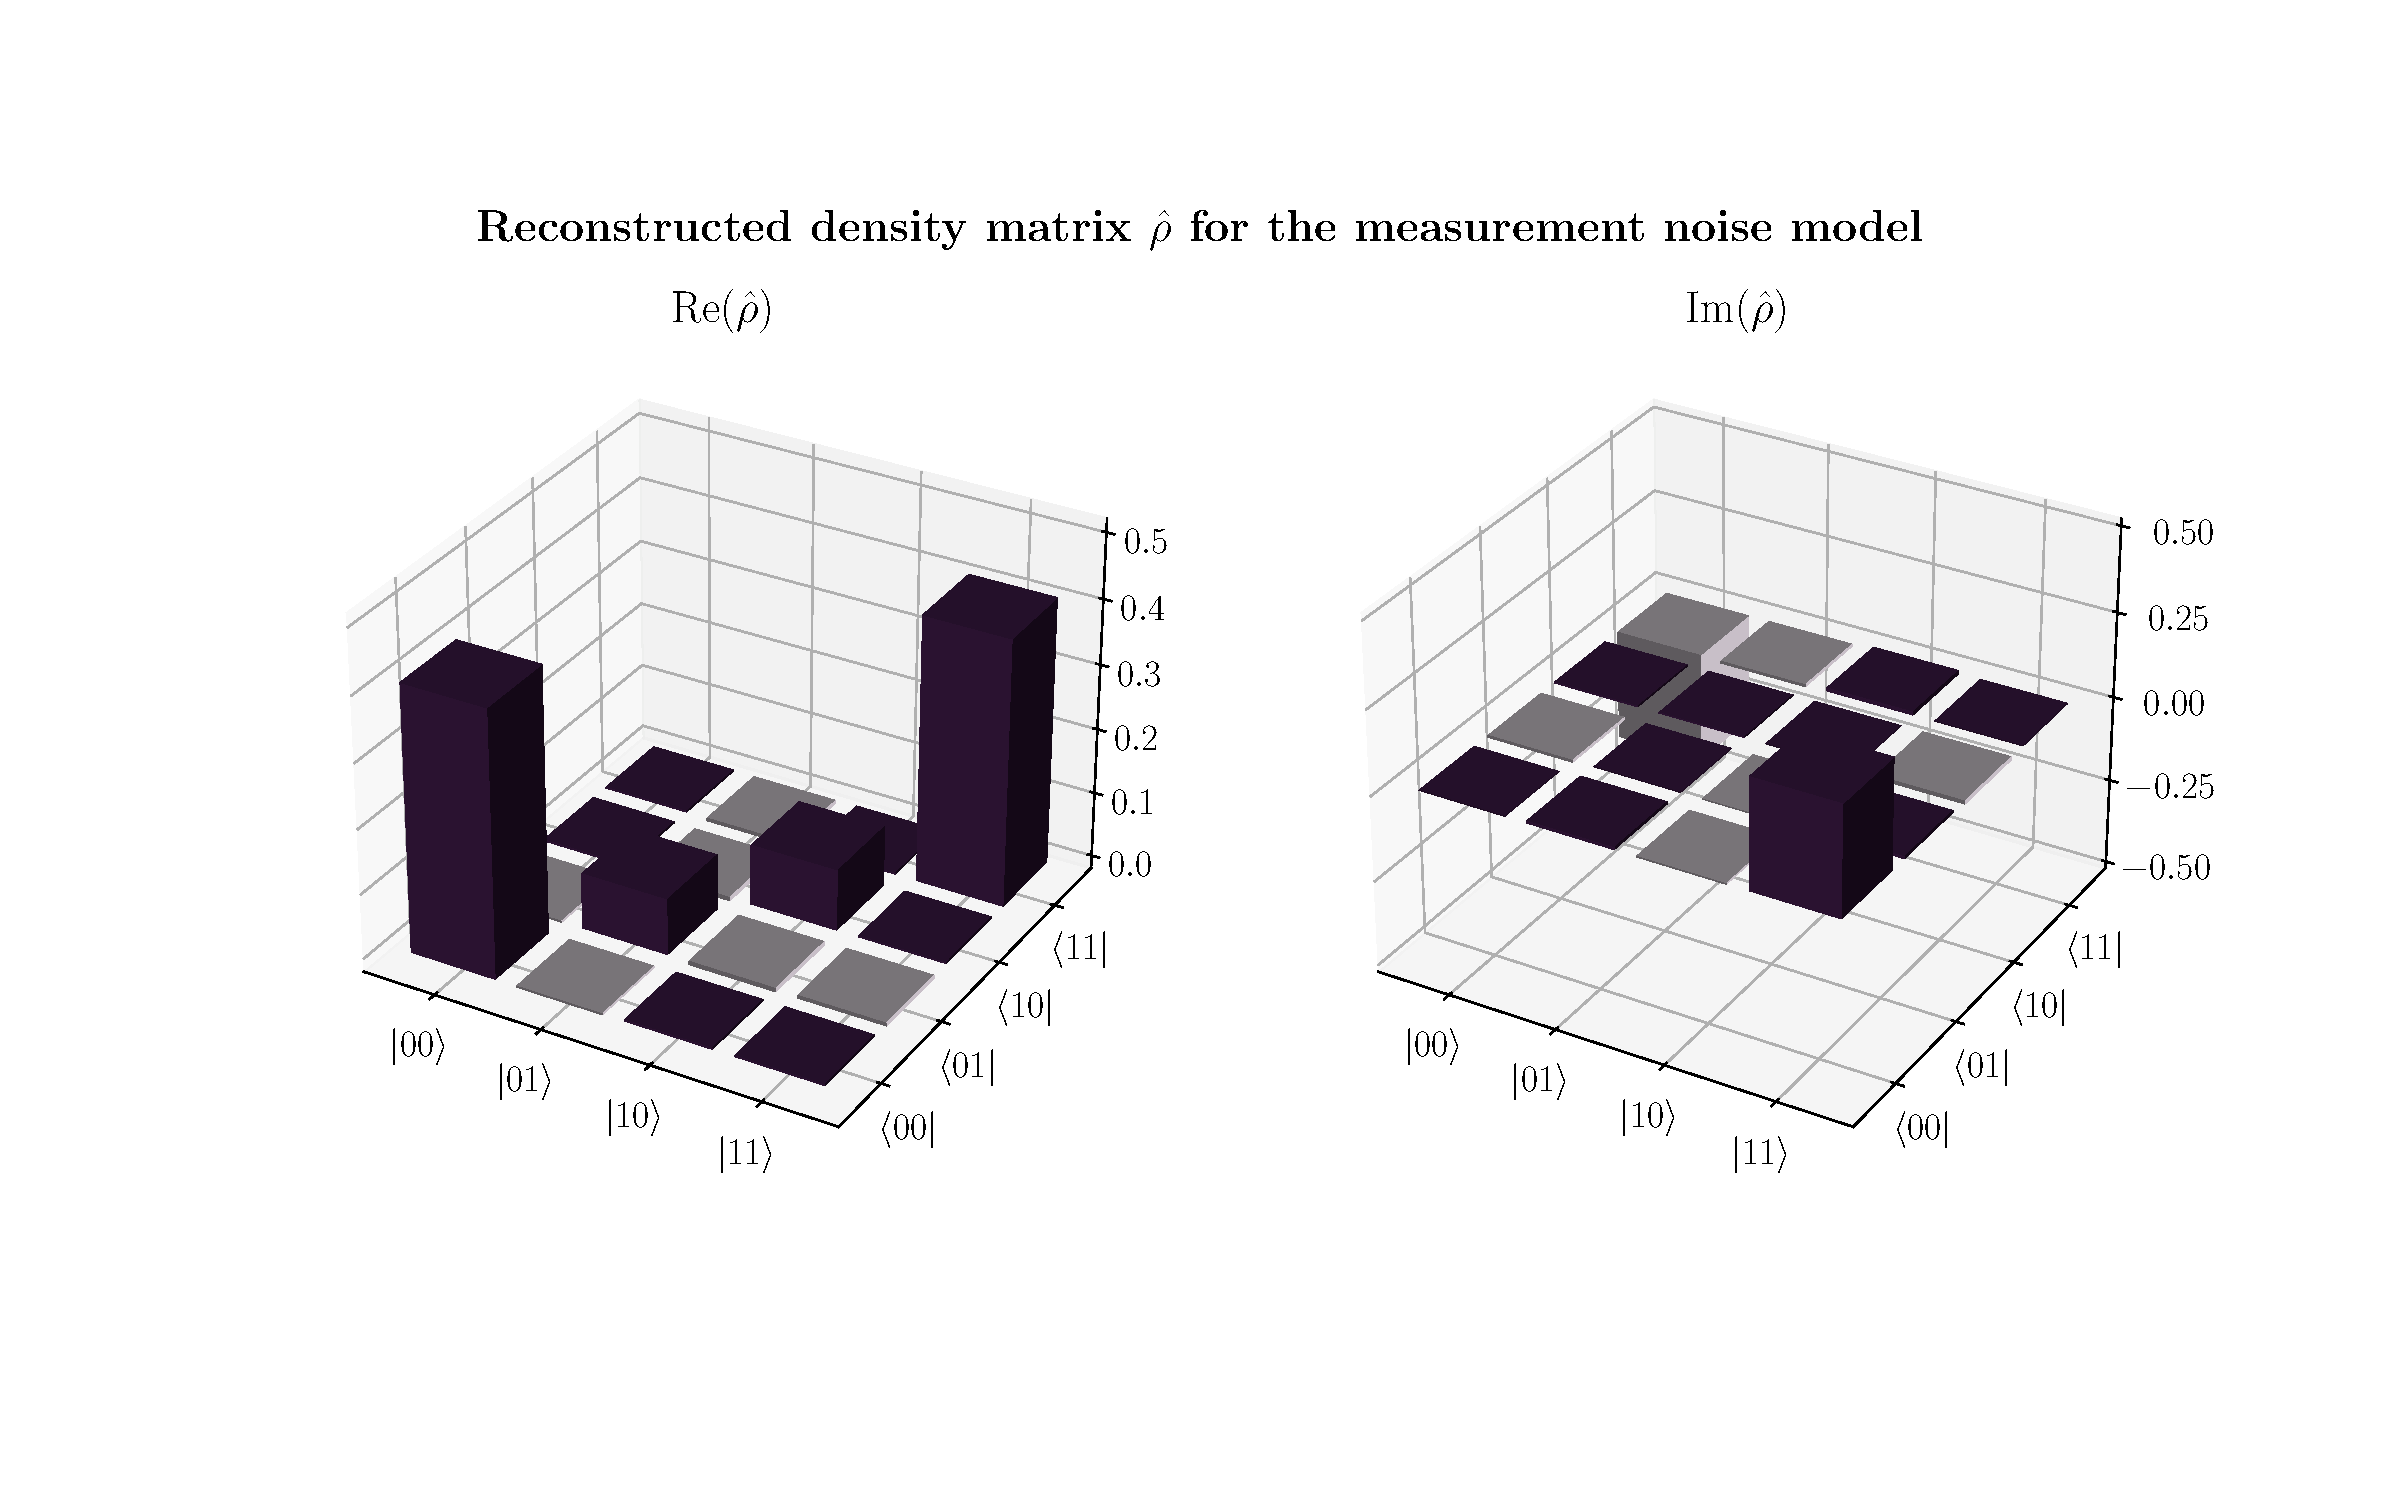
\includegraphics[width=0.9\textwidth, trim={6cm 5cm 3cm 2cm},clip]{figs/density_matrix_meas.pdf}
    \caption{The reconstructed density matrix $\hat{\rho}$ of the entangled two-qubit system after performing the quantum state tomography with measurement noise. In this case, the \texttt{linear\_inversion} fitter was used.}
    \label{fig:meas}
\end{figure}
\vspace{-1cm}
\begin{figure}[H]
    \centering
    \includegraphics[width=0.9\textwidth, trim={6cm 5cm 3cm 2cm},clip]{figs/density_matrix_both.pdf}
    \caption{The reconstructed density matrix $\hat{\rho}$ of the entangled two-qubit system after performing the quantum state tomography with both depolarizing and measurement noise. In this case, the \texttt{linear\_inversion} fitter was used.}
    \label{fig:both}
\end{figure}
\subsection{Parallel Experiments}
Table \ref{tab:parallel} shows the fidelity after performing QST with depolarizing noise on each qubit for the parallel experiments. The corresponding reconstructed density matrices $\hat{\rho}$ are shown in Figures \ref{fig:q1}, \ref{fig:q3}, \ref{fig:q2} and \ref{fig:q4} in Appendix \ref{A}.
\begin{table}[H]
    \centering
    \caption{The fidelity after performing the quantum state tomography with depolarizing noise for the parallel experiments.}
    \begin{tabular}{|l|c|c|}
        \toprule
        \textbf{Qubit(s)} & \textbf{Gate} & \textbf{Fidelity $\mathcal{F}(\hat{\rho}, \hat{\rho}_{\text{exp}})$} \\
        \midrule
        1 & \begin{quantikz}
            & \gate{H} & \qw
        \end{quantikz} & 0.9065 \\
        2 \& 4 & \begin{quantikz}
            & \gate{CX} & \qw
        \end{quantikz} & 0.9258 \\
        3 & \begin{quantikz}
            & \gate{S} & \qw
        \end{quantikz} & 0.9489 \\
        5 & \begin{quantikz}
            & \gate{X} & \qw
        \end{quantikz} & 0.9476 \\ \bottomrule
    \end{tabular}
    \label{tab:parallel}
\end{table}
\vspace{-0.7cm}
\section{Discussion}
Firstly, we notice a substantial decrease of the fidelity when noise is introduced into the system, decreasing significantly from nearly 1 in the noiseless case. This is of course expected, as the noise models change the state of the qubits, which makes the reconstruction harder. For both fitters, we see that the fidelity is slightly lower for the measurement noise model compared to the depolarizing noise model. A possible explanation for this is that the measurement noise model affects the actual measurements, which is the primary source for the tomography algorithm when it tries to reconstruct the density matrix. The depolarizing noise model, on the other hand, only affects the state of the qubits, which is not as crucial for the algorithm. Furthermore, the fidelity is lowest when both noise models are used, which is also expected, as this yields more general noise. 

Moreover, the affect of the noise models can be seen clearly when comparing the ideal state's density matrix in Figure \ref{fig:ideal} with Figures \ref{fig:depol}, \ref{fig:meas} and \ref{fig:both}. As expected, both the depolarizing and measurement noise model significantly increases the diagonal terms in the density matrix. For the depolarizing noise model, this can be understood when studying Equation \ref{depolarizing} which describes the state after depolarizing noise. Here, the first term is proportional to the identity matrix, i.e. it increases the diagonal terms, while the second term reduces the entries of the original state. For the measurement noise model, it is easy to show why the diagonal terms increase. Our ideal output state in Equation \ref{state} will yield two possible noisy outcome states,
\begin{equation}
    \begin{cases}
        \ket{\psi}_1' = \frac{1}{\sqrt{2}}\left(\ket{10} + i\ket{01}\right), \text{ if measurement noise on the 1st qubit} \\
        \ket{\psi}_2' = \frac{1}{\sqrt{2}}\left(\ket{01} + i\ket{10}\right), \text{ if measurement noise on the 2nd qubit.}
    \end{cases}
\end{equation}
After some simple math, one can derive that the corresponding density matrices increase the real parts of the two diagonal terms associated with $\ket{01}$ and $\ket{10}$. In the same way, one will discover that the imaginary parts of these density matrices will cancel out each other, as the result also shows. As a final note, the appearance of the density matrix with both noise models is no surprise, as that is a combination of the two previous cases.

As for the different tomography fitters, we see that the fidelity is slightly higher for the \mintinline{python}|cvxpy_gaussian_lstsq| fitter compared to the \mintinline{python}|linear_inversion| fitter. This is likely due to the more advanced nature of the \mintinline{python}|cvxpy_gaussian_lstsq| fitter, as mentioned earlier. On the other hand, the fitting time is also higher for the \mintinline{python}|cvxpy_gaussian_lstsq| fitter, which is expected for the same reason as above.

Lastly, in the parallel experiments we see that the fidelity is higher in comparison to the experiments with the entangled two-qubit system. This is likely due to the fact that the parallel experiments are performed on separate qubits, which makes the reconstruction easier. As for the density matrices displayed in Appendix \ref{A}, we see a smaller noise impact than in the case of the entangled two-qubit system. Since the gate on each qubit in some cases has little to none effect on the input state, the noise model has less impact on the reconstructed density matrix. For example, the CNOT gate on qubits 2 and 4 only flips the second qubit if the first qubit is in state $\ket{1}$. Since the input state is $\ket{00}$, the gate has no effect on the state, and the noise impact is negligible.

\section{Conclusion}
In this project, we have studied the concept of quantum state tomography on an entangled two-qubit system using different approaches implemented via \texttt{Qiskit}. In the simulations, two different noise models were used to increases the realism of the experiments. In both cases, the fidelity of the reconstructed state decreased significantly, which is expected. Also, the impact of the noise models on the density matrix was clearly visible and in line with the theoretical expectations.

When comparing different tomography fitters, the fidelity was slightly higher for the \mintinline{python}|cvxpy_gaussian_lstsq| fitter compared to the \mintinline{python}|linear_inversion| fitter. However, this came at the cost of a longer fitting time. Lastly, the parallel experiments showed that the fidelity was higher compared to the entangled two-qubit system, which is likely due to the fact that the parallel experiments were performed on separate qubits.

In conclusion, QST is a powerful tool for reconstructing the density matrix of a quantum system. This is essential for verifying quantum states in many applications, including quantum computing and quantum communication. Moreover, parallel experiments can be a useful tool to save time when performing QST on multiple qubits. However, in all cases, it is important to consider the impact of noise and the tomography fitters used, as they can have a significant impact on the results.

\newpage
\printbibliography

\newpage
\appendix
\pagenumbering{roman}
\setcounter{page}{1}
\section{Additional Results} \label{A}
Figures \ref{fig:q1}, \ref{fig:q3}, \ref{fig:q2} and \ref{fig:q4} below show the reconstructed density matrix $\hat{\rho}$ of the entangled two-qubit system after performing QST with depolarizing noise for qubits 1, 2 \& 4, 3 and 5, respectively, during the parallel experiments. The fidelities are shown in Table \ref{tab:parallel}.
\begin{figure}[H]
    \centering
    \includegraphics[width=0.9\textwidth, trim={6cm 5cm 3cm 2cm},clip]{figs/parallel/density_matrix_parexp_0.pdf}
    \caption{The reconstructed density matrix $\hat{\rho}$ of the entangled two-qubit system after performing QST on the first qubit with depolarizing noise in the parallel experiment.}
    \label{fig:q1}
\end{figure}

\begin{figure}[H]
    \centering
    \includegraphics[width=0.9\textwidth, trim={5cm 5cm 3cm 2cm},clip]{figs/parallel/density_matrix_parexp_2.pdf}
    \caption{The reconstructed density matrix $\hat{\rho}$ of the entangled two-qubit system after performing QST on the second and fourth qubit with depolarizing noise in the parallel experiment.}
    \label{fig:q3}
\end{figure}

\begin{figure}[H]
    \centering
    \includegraphics[width=0.9\textwidth, trim={6cm 5cm 3cm 2cm},clip]{figs/parallel/density_matrix_parexp_1.pdf}
    \caption{The reconstructed density matrix $\hat{\rho}$ of the entangled two-qubit system after performing QST on the third qubit with depolarizing noise in the parallel experiment.}
    \label{fig:q2}
\end{figure}

\begin{figure}[H]
    \centering
    \includegraphics[width=0.9\textwidth, trim={6cm 5cm 3cm 2cm},clip]{figs/parallel/density_matrix_parexp_3.pdf}
    \caption{The reconstructed density matrix $\hat{\rho}$ of the entangled two-qubit system after performing QST on the fifth qubit with depolarizing noise in the parallel experiment.}
    \label{fig:q4}
\end{figure}

\section{Notes on AI Assistance}
The text in this report is my own work. However, some parts of the project source code was generated with the help of GitHub Copilot. This includes the function for plotting the density matrix and basic functions for saving and loading data. Although, I have reviewed and modified the generated code to fit my goals.

\end{document}